\documentclass[conference]{IEEEtran}
\IEEEoverridecommandlockouts%The preceding line is only needed to identify funding in the first footnote. If that is unneeded, please comment it out.

\usepackage[utf8]{inputenc}
\usepackage{cite}
\usepackage{amsmath,amssymb,amsfonts}
\usepackage{algorithmic}
\usepackage{graphicx}
\usepackage{textcomp}
\usepackage{xcolor}
\usepackage{lipsum}


\def\BibTeX{{\rm B\kern-.05em{\sc i\kern-.025em b}\kern-.08em
    T\kern-.1667em\lower.7ex\hbox{E}\kern-.125emX}}

%Para justificar sin cortar palabras
\tolerance=1
\emergencystretch=\maxdimen
\hyphenpenalty=10000
\hbadness=10000

%-------------------------------------------------------------------------------
%	BEGIN DOCUMENT
%-------------------------------------------------------------------------------
\begin{document}

%-------------------------------------------------------------------------------
%	DOCUMENT INFORMATION
%-------------------------------------------------------------------------------
\title{Tarea 2 - Dithering\\
%{\footnotesize \textsuperscript{*}Note: Sub-titles are not captured in Xplore and should not be used}
%\thanks{Identify applicable funding agency here. If none, delete this.}
}


%-------------------------------------------------------------------------------
%	AUTHORS
%-------------------------------------------------------------------------------
\author{
\IEEEauthorblockN{Daniel Torres Robledo}
\IEEEauthorblockA{\textit{shadow.cat6333@gmail.com}}
\and
\IEEEauthorblockN{Andrés Fuentes Hernández}
\IEEEauthorblockA{\textit{andres7233@hotmail.com}}

}

\maketitle


%-------------------------------------------------------------------------------
%	ABSTRACT
%-------------------------------------------------------------------------------
\begin{abstract}
En este documento se aborda el tema de \textit{dithering}, mostrando la implementación de \textit{dither ordenado}, \textit{dither aleatorio} y \textit{dither difusión de error}, para éste último en escala de grises y color.
\end{abstract}

\begin{IEEEkeywords}
dithering, Floyd Steinberg, random, ordered, shared error, python, opencv
\end{IEEEkeywords}

%-------------------------------------------------------------------------------
%	INTRODUCTION
%-------------------------------------------------------------------------------
\section{Introducción}

El uso del \textit{dithering} permite poder mostrar imágenes en formatos que tengan una cantidad menor de color de profundidad, que para el caso de esta tarea, será 1 bit.

Esta técnica es empleada en las impresiones de periódicos o formatos en donde se tiene solo una tinta o color de profundidad de 1 bit, para lograr obtener una mayor resolución radiométrica, pero a su vez sacrificando resolución espacial, esto se logra aprovechando la integración espacial dentro del ojo humano\cite{b1}.

El objetivo es mostrar las diferencias entre algunas implementaciones de \textit{dithering}, que son: \textit{dither ordenado}, \textit{dither aleatorio} y \textit{dither difusión de error}. Con variaciones en parámetros de algunas de éstas y una versión en color de difusión de error.


%-------------------------------------------------------------------------------
%	SECTION 1
%-------------------------------------------------------------------------------
%\section{\textit{Dithering}}
%\textcolor{violet}{\lipsum[3]}
%
%%-------------------------------------------------------------------------------
%\subsection{Ventajas}
%\textcolor{violet}{\lipsum[3]}
%
%%-------------------------------------------------------------------------------
%\subsection{Desventajas}
%\textcolor{violet}{\lipsum[3]}


%-------------------------------------------------------------------------------
%	SECTION 2
%-------------------------------------------------------------------------------
\section{Implementación}

Para ésta práctica se utilizó \textit{python}, con las bibliotecas de \textit{opencv, numpy, scipi  y skimage}.

A continuación se describen características de cada uno de los métodos implementados y se muestran imágenes resultantes de aplicar dicho método.


%-------------------------------------------------------------------------------
\subsection{\textit{Random Dithering}}

Esta variante de \textit{dithering} es la más sencilla de implementar, sin embargo los resultados generalmente son los peores de las implementaciones. Se puede observar en la figura \ref{random} la  imagen original y la resultante.

\begin{figure}[htbp]
\centerline{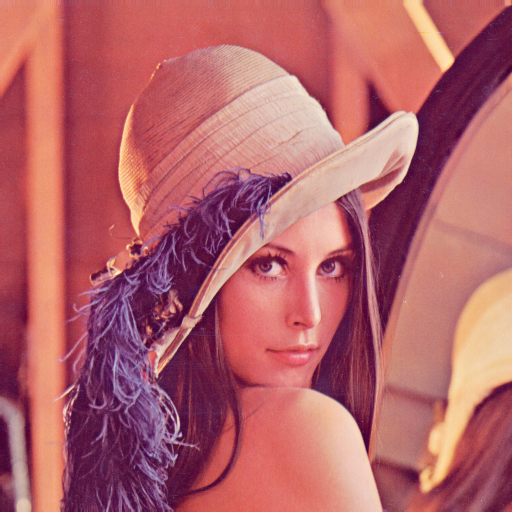
\includegraphics[height=50mm]{code/lena}}
\centerline{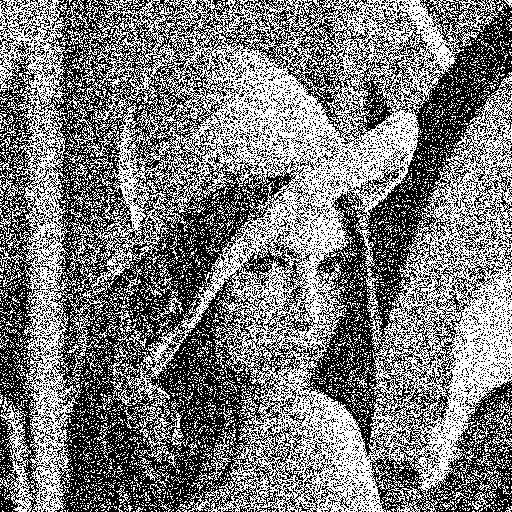
\includegraphics[height=50mm]{code/random_dither_lena}}
\caption{Ejemplo de \textit{random dither}.}
\label{random}
\end{figure}

Se puede observar que tanto en partes oscuras y claras hay puntos negros y blancos, por lo que esta técnica agrega mucho ruido al resultado.

A continuación se muestra el código de este método:

\begin{figure}[htbp]
\centerline{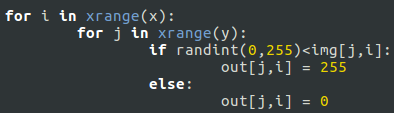
\includegraphics[width=80mm]{code/random_dither}}
\caption{Código para \textit{random dither}.}
\label{randomPy}
\end{figure}


%-------------------------------------------------------------------------------
\subsection{\textit{Ordered Dithering}}

En esta técnica se utilizan matrices de $N\times N$ donde cada pixel de la imagen original es mapeado por la operación módulo $N$ a la matriz definida, también es importante mencionar que el valor de cada pixel se escala de sus posibles valores en $[0,255]$ a un intervalo de $[0,N]$ para poder comparar con los valores de la matriz, en donde si es menor o igual el resultado es $0$, en otro caso es en $1$.

Para este ejemplo, se utilizarán tres matrices, las cuales son\cite{b3}:

$d_2=\begin{matrix}
	3 & 1\\
	0 & 2
\end{matrix}$
$d_3=\begin{matrix}
	0 & 7 & 3\\
	6 & 5 & 2\\
	4 & 1 & 8\\
\end{matrix}$
$d_4=\begin{matrix}
	0 & 8 & 2 & 10\\
	12 & 4 & 14 & 6\\
	3 & 11 & 1 & 9\\
	15 & 7 & 13 & 5\\
\end{matrix}$

\begin{figure}[htbp]
\centerline{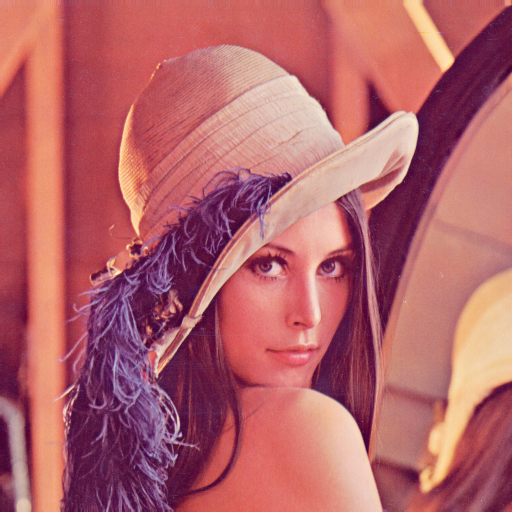
\includegraphics[height=50mm]{code/lena}}
\centerline{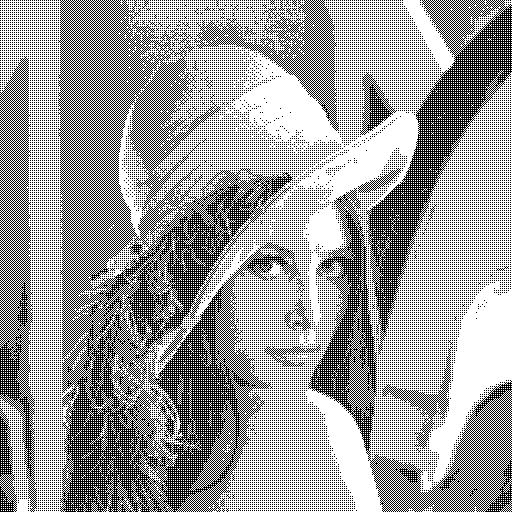
\includegraphics[height=50mm]{code/ordered_dither_2_lena}}
\centerline{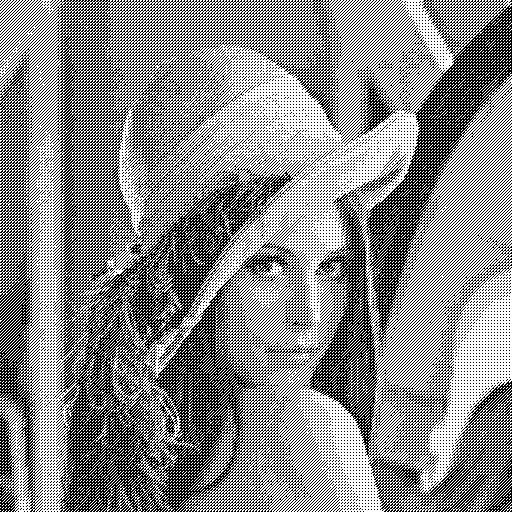
\includegraphics[height=50mm]{code/ordered_dither_3_lena}}
\centerline{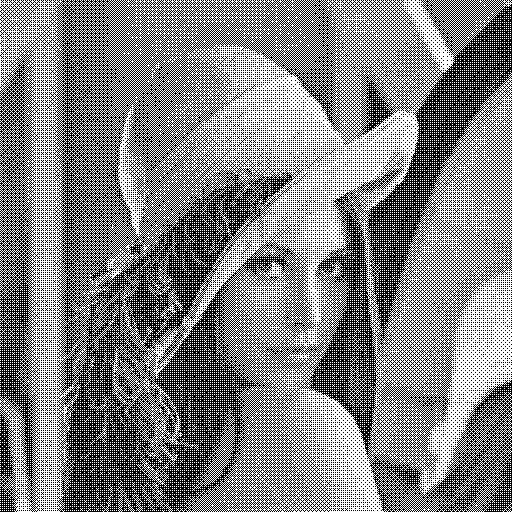
\includegraphics[height=50mm]{code/ordered_dither_4_lena}}
\caption{Ejemplo de \textit{ordered dither} utlizando las matrices d2, d3, d4.}
\label{ordered}
\end{figure}

En la figura \ref{ordered}, se pueden observar los diferentes resultados de la misma imagen utilizando este método con diferentes tamaños de matrices, en orden de arriba a abajo d2, d3, d4.

Donde se puede observar que matrices más grandes generan mejores resultados. Pero una desventaja es que los patrones de las matrices son visibles, sobre todo en matrices pequeñas.

A continuación se muestra el código de este método:

\begin{figure}[htbp]
\centerline{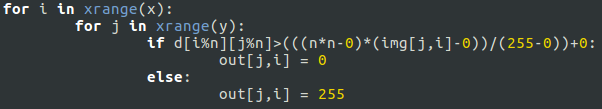
\includegraphics[width=80mm]{code/ordered_dither}}
\caption{Código para \textit{random dither}.}
\label{orderedPy}
\end{figure}

%-------------------------------------------------------------------------------
\subsection{\textit{Shared Error Dithering Color}}
El método de \textit{Floyd Steinberg} para \textit{dithering}, es un método de difusión del error
y surge debido a que otros métodos de \textit{dithering} como el ordenado dependen de crear 
una matriz $N\times N$ en la que se utilizan patrones de cuadros blancos y negros que 
emulan las escalas de grises, estos métodos tienen como consecuencia la perdida 
de resolución o bien una imagen de salida con dimensiones superiores a la original.
Este método que surgió en el año de 1976, cuyo propósito es mantener el mismo tamaño de imagen repartiendo el error generado al binarizar ese pixel hacia los pixeles vecinos, pero solo aquellos
\textit{adelante} y por \textit{debajo} de el es decir no se repartirá el error a pixeles ya visitados.

%Se utilizó el algoritmo de Floyd Steinberg para las 3 capas de color R,G,B para así obtener un
%\textit{dithering }en 3 dimensiones. El programa es el siguiente:

Para observar el comportamiento de este método se eligieron 3 imágenes, Lena, un bosque y
una imagen artificial de triángulos y colores. En la figura \ref{errorColorLena}
%imagen de lena Fig1
se puede observar que la imagen con \textit{dithering} es una buena representación de la original, en donde  los rasgos del rostro humano se pueden distinguir fácilmente, también es posible notar ciertos patrones en forma de \textit{grecas} aparecen en la imagen esto puede deberse a la forma en la que el algoritmo distribuye el ruido.


%Fig1.jpg  Fig2.jpg

\begin{figure}[htbp]
\centerline{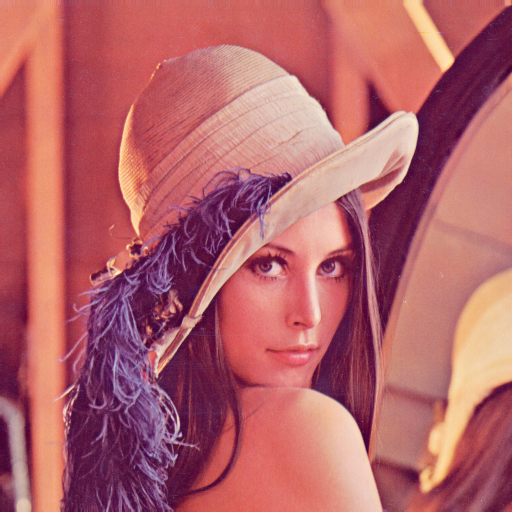
\includegraphics[height=50mm]{code/lena}}
\centerline{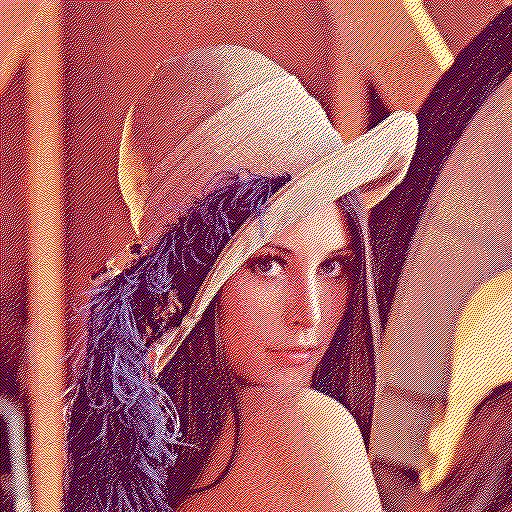
\includegraphics[height=50mm]{code/Fig1}}
\caption{Ejemplo de \textit{shared error dither} con Lena.}
\label{errorColorLena}
\end{figure}

También se utilizó una imagen de un bosque, ya que se quería ver si los detalles de las hojas de los pinos se preservaban en la imagen con \textit{dithering}, además esta imagen tiene un brillo en la esquina superior izquierda.

En la figura \ref{errorColorTree} se puede ver que una gran porción de la imagen es blanca debido al brillo sin embargo los pinos y algunos de sus detalles aun se pueden distinguir con facilidad, incluso el paisaje de fondo ,el cual en la imagen original  esta desenfocado y tiene un alto brillo, es posible distinguirlo en la imagen con \textit{dithering}

%Fig3 Fig 4

\begin{figure}[htbp]
\centerline{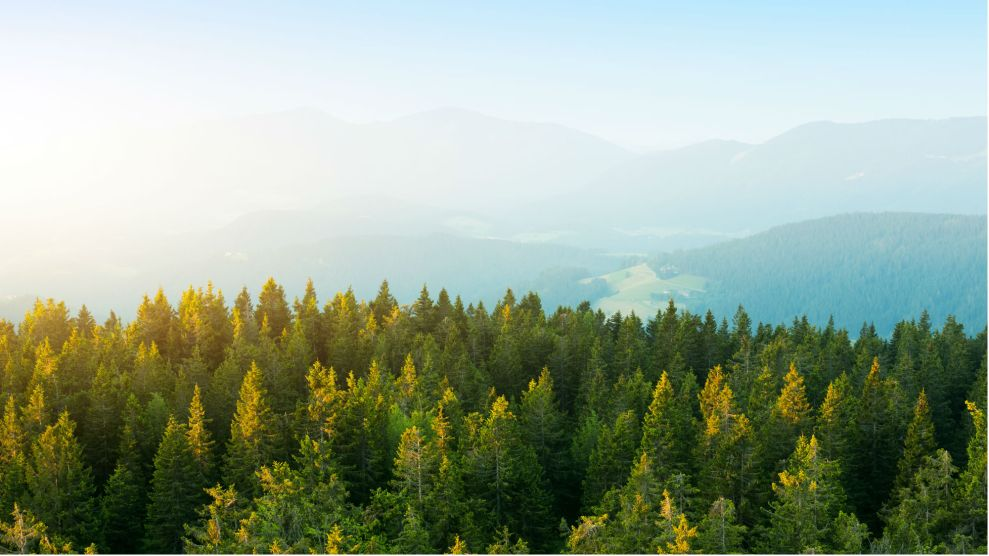
\includegraphics[height=50mm]{code/bosque}}
\centerline{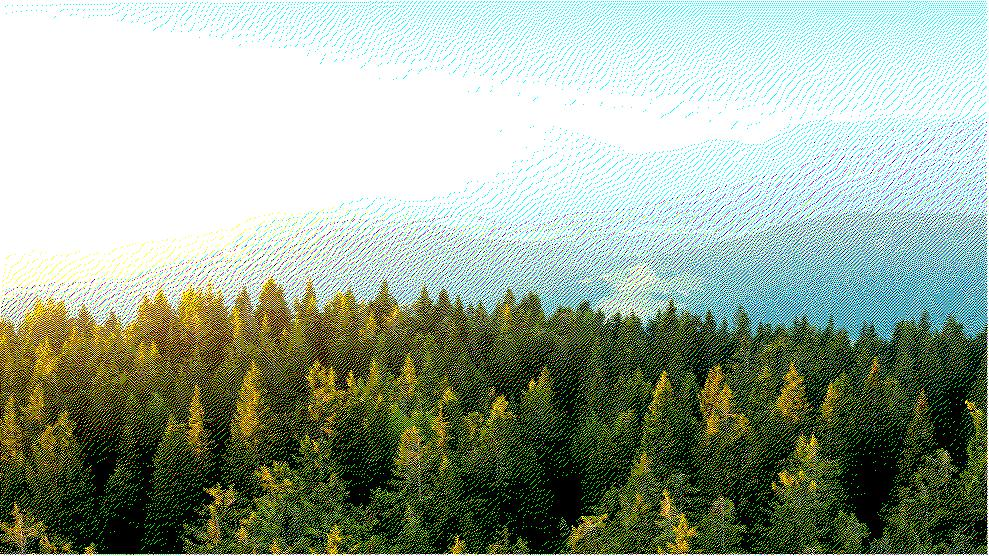
\includegraphics[height=50mm]{code/bosque1}}
\caption{Ejemplo de \textit{shared error dither} con el bosque.}
\label{errorColorTree}
\end{figure}


Finalmente el algoritmo se puso a prueba con una imagen artificial es decir no es la representación
de nuestro mundo. La última prueba consiste de una serie de triángulos de diferentes colores, el objetivo de  esta prueba es ver la eficiencia del algoritmo con color uniformes y en los contornos. En la figura \ref{errorColorTriangle} se puede observar de una manera mas clara el ruido en forma de "grecas" y en general aunque la imagen asemeja la original tiene un ruido significativo. Los triángulos mas afectados por este ruido son aquellos de color claro que se encuentran junto a un color mas obscuro. Es posible observar  franjas del color adyacente en dichos triángulos.

\begin{figure}[htbp]
\centerline{
\includegraphics[height=50mm]{code/colors}}
\centerline{
\includegraphics[height=50mm]{code/colors1}}
\caption{Ejemplo de \textit{shared error dither} con triángulos.}
\label{errorColorTriangle}
\end{figure}

%-------------------------------------------------------------------------------
\subsection{\textit{Shared Error Dithering}}

Esta implementación, al igual que la anterior, pero en un solo canal y un bit de profundidad, se puede apreciar un resultado con calidad similar al de \textit{Ordered Dither} de una matriz de $4\times 4$, sin embargo, aquí no hay patrones visibles.

\begin{figure}[htbp]
\centerline{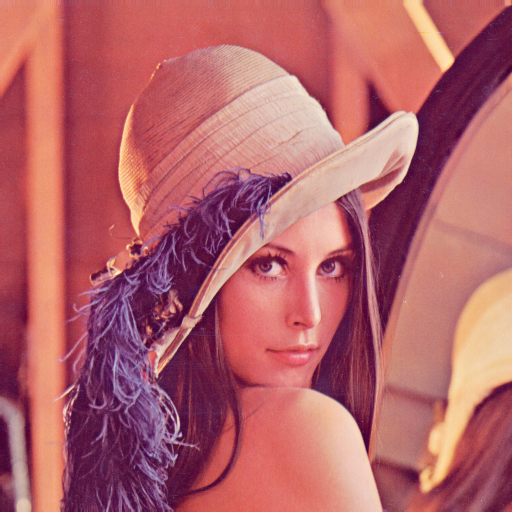
\includegraphics[height=50mm]{code/lena}}
\centerline{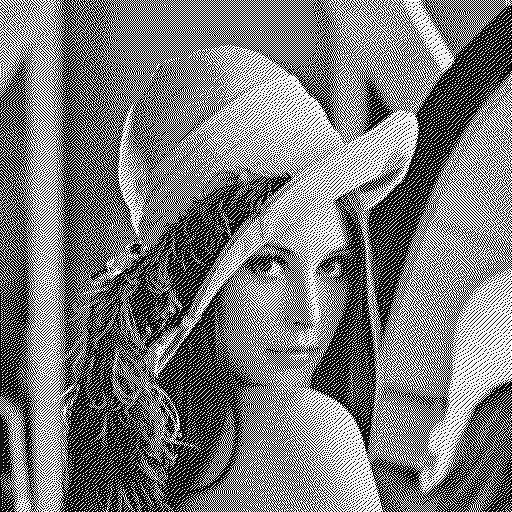
\includegraphics[height=50mm]{code/error_dither_lena}}
\caption{Ejemplo de \textit{shared error dither} en 1 bit.}
\label{errorGray}
\end{figure}

Sin embargo, este algoritmo es el que tarda más en ejecutarse pero ofrece resultados buenos, manteniendo características de la imagen, como los bordes del sombrero y partes de las plumas del mismo.
A continuación se muestra el código de este método:

\begin{figure}[htbp]
\centerline{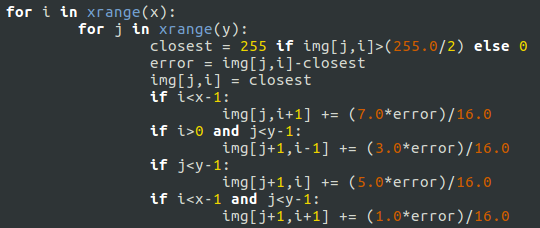
\includegraphics[width=80mm]{code/error_dither}}
\caption{Código para \textit{random dither}.}
\label{esrrorPy}
\end{figure}

%-------------------------------------------------------------------------------
%	SECTION 2
%-------------------------------------------------------------------------------
\section{Conclusiones}

En general, los diferentes métodos de \textit{dithering} implementados muestran resultados donde se puede apreciar la imagen original con al menos unos detalles.

El peor de los métodos fue el aleatorio, donde la imagen resultante tiene mucho ruido.

Posteriormente, el \textit{dither} ordenado muestra un buen desempeño, pero depende de poder crear las matrices de $N \times N$, mientras más grande sea $N$, los resultados son mejores, sin embargo, los patrones de estas matrices son claros a simple vista.

El algoritmo de \textit{Floyd Steinberg}  para \textit{dithering} produce una buena aproximación a la imagen original utilizando solo 1 bit por color. Aunque aun es posible ver ciertos patrones sobre todo en lugares de color uniforme que tienen vecindad con un color mas obscuro, cierta \textit{contaminación} se puede producir.

Este último algoritmo muestra los mejores resultados, preservando suficientes detalles de la imagen original, sin embargo el tiempo de procesamiento es el mayor de todos.

Por lo que se recomienda \textit{Shared Error Dithering} para generar este tipo de imágenes cuando el dispositivo en donde se visualizará tiene solo un color, sin embargo si lo que se busca es velocidad de respuesta \textit{Ordered Dithering} es una buena opción, con una matriz de tamaño 3 o 4.


%-------------------------------------------------------------------------------
%	BIBLIOGRAPHY
%-------------------------------------------------------------------------------
\begin{thebibliography}{00}
\bibitem{b1} Team Veryovka-Buchanan, \textit{Developed Algorithms}. Avalible at \textit{https://www.visgraf.impa.br/Courses/ip00/proj/Dithering1/\\algoritmos\_desenvolvidos.htm}. [Accessed Agosto 25, 2019]

\bibitem{b2} Tanner Helland, \textit{Image Dithering: Eleven Algorithms and Source Code}. Avalible at \textit{http://www.tannerhelland.com/4660/dithering-eleven-algorithms-source-code}. [Accessed Agosto 25, 2019]

\bibitem{b3} Ordered Dithering. [Online]. Avalible at \textit{https://en.wikipedia.org/wiki/Ordered\_dithering}. [Accessed Agosto 25, 2019]
\end{thebibliography}

%\vspace{12pt}
%\color{red}
%IEEE conference templates contain guidance text for composing and formatting conference papers. Please ensure that all template text is removed from your conference paper prior to submission to the conference. Failure to remove the template text from your paper may result in your paper not being published.

%-------------------------------------------------------------------------------
%	END DOCUMENT
%-------------------------------------------------------------------------------
\end{document}